\chapter{Input Data}
\section{Problem 1: Simple network}
In the first problem a small neural network with 4 Layers was provided.
\begin{figure}[h]
	\centering
	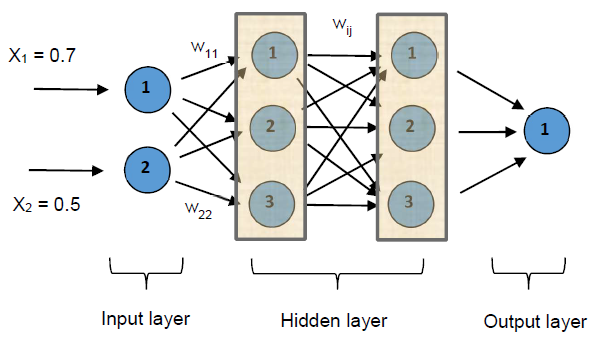
\includegraphics[height=8cm]{img/nn_task1.png}
	\caption{Simple neural network for problem 1}
    \label{nn_task1}
\end{figure}
In addition the input values and the weights for the connections of the fully connected layers were provided.
\begin{figure}[h]
	\centering
	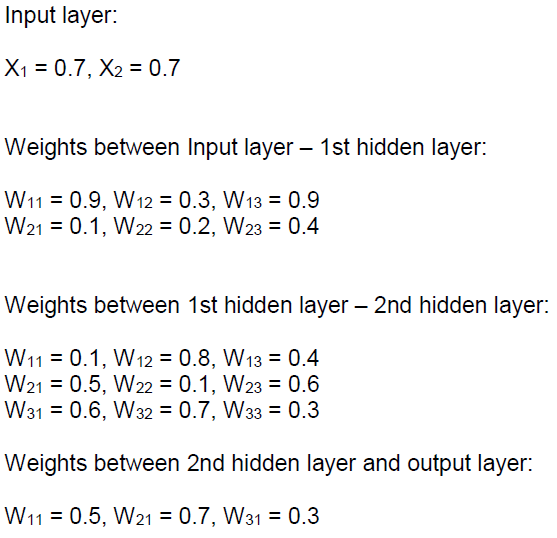
\includegraphics[height=8cm]{img/data_task1.png}
	\caption{Data provided for problem 1}
    \label{data_task1}
\end{figure}
\section{Problem 2: Backpropagation}
Similarly to the first problem a small neural network was provided, in this case the network consists only of a single neuron with two inputs and an activation function $Z$.
\begin{figure}[t]
	\centering
	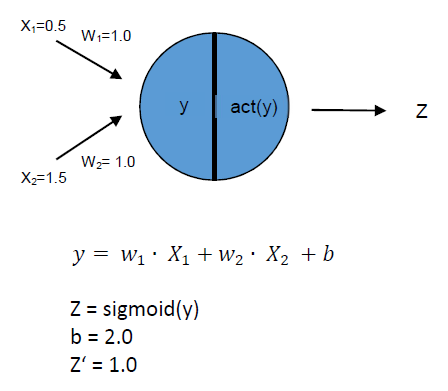
\includegraphics[height=8cm]{img/nn_task2.png}
	\caption{Single neuron for problem 2}
    \label{nn_task1}
\end{figure}

\section{Problem 3: Artificial neural network}
For the third problem a small neural network with 3 Layers was provided in form of a python script using the Pytorch library, in addition to the network a dataset called \textbf{One-hundred plant species leaves data set Data Set}. This dataset contains the leaves of 100 different plant species each represented with 16 examples of real leaves, which are themselves represented by a feature vector with 64 different elements representing different features.

\section{Problem 4: Gradient Descent}

The input data set consists of 1000 generated points with a $X$ value between $-5$ and $5$.
The $Y$ value is calculated with the formula $ y = mx + c $ where $m$ and $c$ are assumed by us.
Applying a random noise leads to the dataset which is shown in Figure \ref{problem4_imput_data}

\begin{figure}[h]
	\centering
	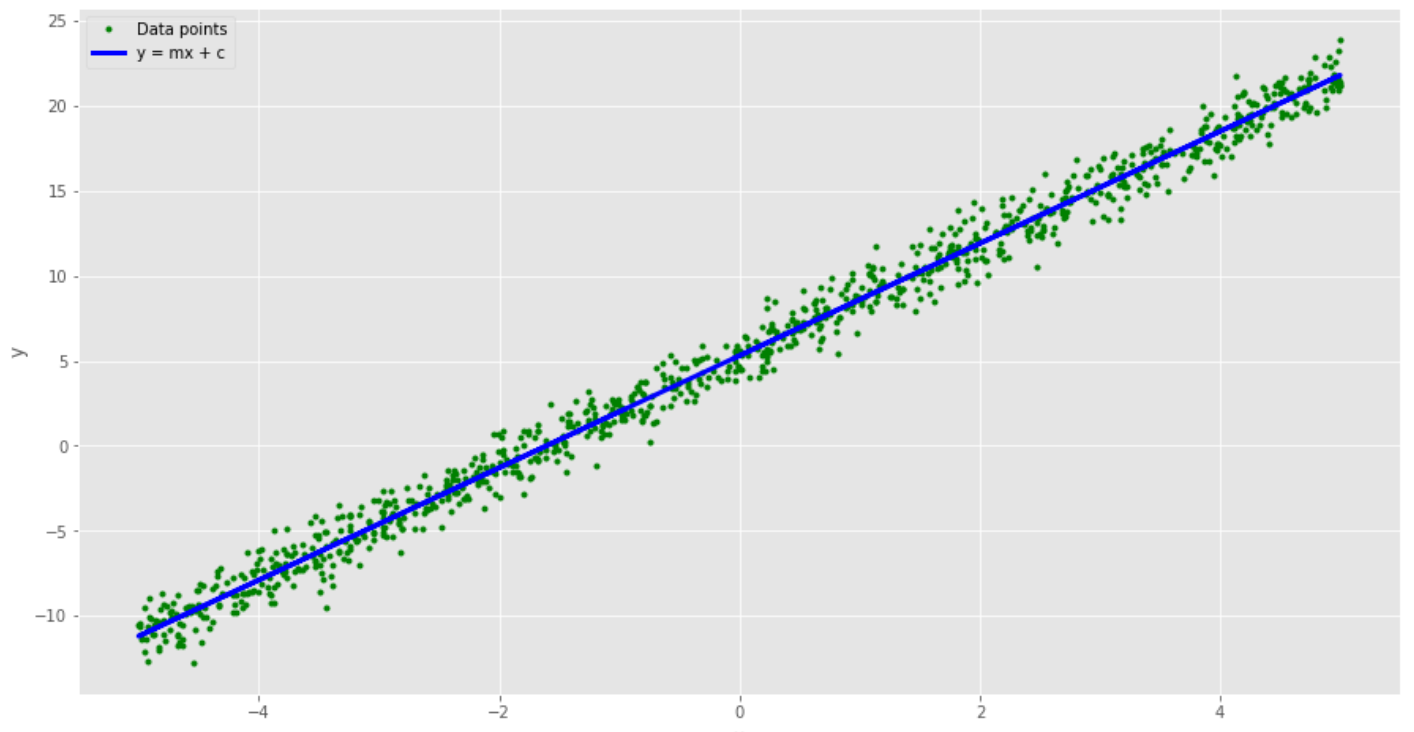
\includegraphics[height=8cm]{img/problem4_imput_data.png}
	\caption{Generated input data of problem 4}
    \label{problem4_imput_data}
\end{figure}

Further a jupyter notebook is provided which generate these data and provides a script which only need to be completed with the calculation of the gradient and updating and weight update for $m$ and $c$.

It is also given that all data points should satisfy this equation.

\begin{equation}\label{gradients1}
    y = mx + c
\end{equation}


